\documentclass{article}
\usepackage{graphicx} % Required for inserting images

\title{Detection of base-pair mismatch in DNA via graphene nanopores}
\author{Sukalyan Deb }
\date{December 2024}

\begin{document}

\maketitle

\section*

The field of quantum transport in DNA begins with a fundamental question: Is DNA a metal, insulator, or semiconductor .For the first time in 1961, D.D. Eley, in his paper, studied the DC conductivity of wheat germ DNA, herring sperm DNA, and Penicillium DNA and he observed a very small departure from Ohm's law. Eley took the first initiative, paving the way for an entirely new and intriguing area of research called quantum transport of DNA. \\

DNA, the basic building block of life is composed of four nitrogenous bases (A, T, G and C), forms a double helix with complementary base pairing (A-T, G-C). The two nitrogen bases of a given pair are connected via a hydrogen bond, whereas different bases are connected via covalent bonds that form the tow rungs of the double-helix. The sequence of the different bases along the rungs is vital, as it controls different biological processes, e.g., DNA replication, transcription, and protein synthesis in living organisms. Any mismatch in DNA base-pairing can cause several epigenetic disorders, including cancer.

\begin{figure}
    \centering
    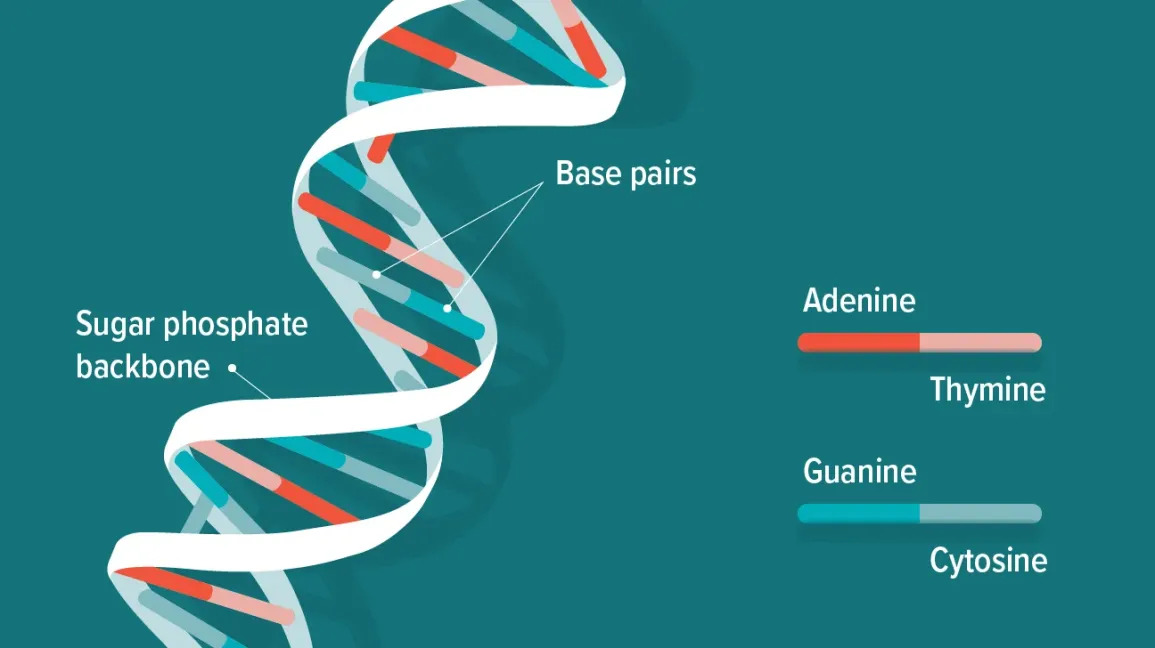
\includegraphics[width=0.7\linewidth]{DNA-01.jpg}
    \caption{DNA}
    \label{fig:enter-label}
\end{figure}


In 1998, at Delft University of Technology, Cees Dekker and his team conducted a groundbreaking  experimental measurement of DNA conductivity. They used double-stranded poly(G)-poly(C) DNA, which is 10.4 nm long and consists of 30 base pairs, placed between platinum-coated electrodes at room temperature. Poly(G)-poly(C) DNA refers to DNA with a significantly higher number of G/C base pairs compared to A/T base pairs.\\

\begin{figure}
    \centering
    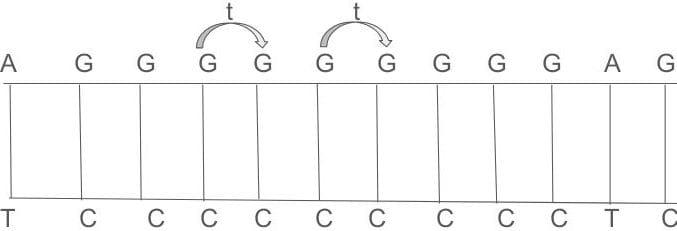
\includegraphics[width=1\linewidth]{WhatsApp Image 2025-01-23 at 17.19.59.jpeg}
    \caption{Schematic diagram of a ds-DNA modeled within a tight-binding framework with hopping parameter 't'.}
    \label{fig:enter-label}
\end{figure}

\begin{figure}
    \centering
    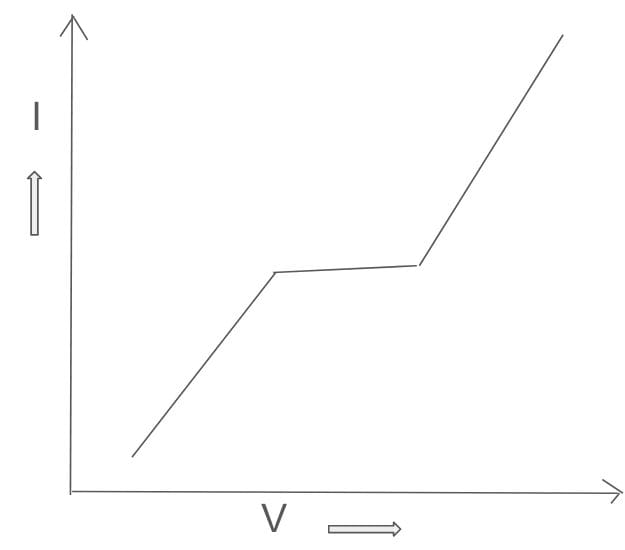
\includegraphics[width=0.5\linewidth]{WhatsApp Image 2025-01-16 at 20.30.30.jpeg}
    \caption{I - V response of the poly(G)-poly(C) DNA showing semiconducting behavior}
    \label{fig:enter-label}
\end{figure}

It was observed that below a certain threshold voltage, the DNA behaved as an insulator, conducting very little current. However, above the threshold voltage, it exhibited decent conductivity. The I-V response curve revealed nonlinear behavior, indicating the presence of a bandgap. Interest in this field surged around 2000, marking a significant milestone in bioelectronics.\\

In condensed matter physics, DNA can be modeled as an extended tight-binding system. The Hamiltonian for DNA includes hopping terms along the rungs of the double-helix, following the covalent bonds. "Hopping" refers to the movement of electrons to their nearest neighbors, representing the kinetic energy terms. Experiments revealed that current flows through the $\pi$-stacked bases along the rungs of the double-helix.\\

\begin{figure}
    \centering
    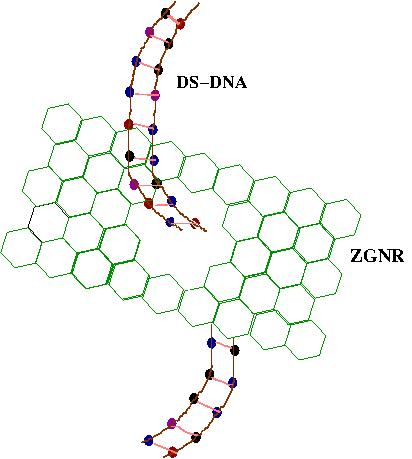
\includegraphics[width=0.5\linewidth]{ds_dna.jpg}
    \caption{Schematic view of the dsDNA passing through the nanopore.}
    \label{fig:enter-label}
\end{figure}

The second mathematical model introduces inter-layer connections between the nitrogenous bases of two rungs, with sugar-phosphate backbones attached with the nitrogen bases along the two helices of the DNA. Sourav and coworkers expanded on this by incorporating both nearest-neighbor and inter-layer hopping between the nitrogen bases of the two helices in their analysis.\\

They examined changes in local density of states, conductivity and I-V characteristics by inserting a ds-DNA chain into a graphene nanopore.The advantage of using graphene nanopores is that it is a unique and more cost-effective technique for DNA sequencing. The results revealed distinct patterns for specific base-pairs including several mismatches. Green's function formalism was used to compute transport properties, including conductance and density of states profiles.\\

Their study explores techniques for detecting DNA base-pair mismatches through conductance and I-V response analysis. They had successfully identified unique signatures related to base-pair mismatches that can lead to different
genetic diseases, offering significant potential to advance genetic and medical diagnostics. This work could also enable a fast and cost-effective DNA sequencing device in the future.\\

\begin{figure}
    \centering
    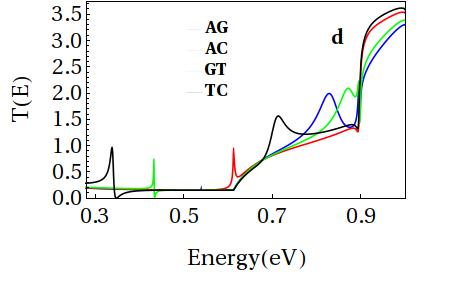
\includegraphics[width=1\linewidth]{trans_4.jpg}
    \caption{Conductance as a function of energy (E) for a ds-DNA with mismatches}
    \label{fig:enter-label}
\end{figure}\\

\section*{References}
(1)Sourav Kundu and S N Karmakar, Nanotechnology \textbf{27} 135101 (2016)\\
(2)J.Watson and F.Crick, Nature(London)
 \textbf{171},737(1953)\\
 (3)Porath D, Bezryadin A, de Vries S, Dekker C. Direct measurement of electrical transport through DNA molecules. Nature. 2000 Feb 10;403(6770):635-8. doi: 10.1038/35001029. PMID: 10688194.\\
 (4)Eley, D. D., & Spivey, D. I. (1962). Semiconductivity of organic substances. Part 9.—Nucleic acid in the dry state. Transactions of the Faraday Society, 58(0), 411–415.
\end{document}
